%%%%%%%%%%%%%%%%%%%%%%%%%%%%%%%%%%%%%%%%%
% Beamer Presentation
% LaTeX Template
% Version 1.0 (10/11/12)
%
% This template has been downloaded from:
% http://www.LaTeXTemplates.com
%
% License:
% CC BY-NC-SA 3.0 (http://creativecommons.org/licenses/by-nc-sa/3.0/)
%
%%%%%%%%%%%%%%%%%%%%%%%%%%%%%%%%%%%%%%%%%

%----------------------------------------------------------------------------------------
%	PACKAGES AND THEMES
%----------------------------------------------------------------------------------------

\documentclass{beamer}
 \usepackage[croatian]{babel}
 \usepackage{subcaption}
 \usepackage{tabularx}
 \usepackage{tikz,}
\mode<presentation> {

% The Beamer class comes with a number of default slide themes
% which change the colors and layouts of slides. Below this is a list
% of all the themes, uncomment each in turn to see what they look like.

%\usetheme{default}
%\usetheme{AnnArbor}
%\usetheme{Antibes}
%\usetheme{Bergen}
%\usetheme{Berkeley}
%\usetheme{Berlin}
%\usetheme{Boadilla}
%\usetheme{CambridgeUS}
%\usetheme{Copenhagen}
%\usetheme{Darmstadt}
%\usetheme{Dresden}
%\usetheme{Frankfurt}
%\usetheme{Goettingen}
%\usetheme{Hannover}
%\usetheme{Ilmenau}
%\usetheme{JuanLesPins}
%\usetheme{Luebeck}
\usetheme{Madrid}
%\usetheme{Malmoe}
%\usetheme{Marburg}
%\usetheme{Montpellier}
%\usetheme{PaloAlto}
%\usetheme{Pittsburgh}
%\usetheme{Rochester}
%\usetheme{Singapore}
%\usetheme{Szeged}
%\usetheme{Warsaw}

% As well as themes, the Beamer class has a number of color themes
% for any slide theme. Uncomment each of these in turn to see how it
% changes the colors of your current slide theme.

%\usecolortheme{albatross}
%\usecolortheme{beaver}
%\usecolortheme{beetle}
%\usecolortheme{crane}
%\usecolortheme{dolphin}
%\usecolortheme{dove}
%\usecolortheme{fly}
%\usecolortheme{lily}
%\usecolortheme{orchid}
%\usecolortheme{rose}
%\usecolortheme{seagull}
%\usecolortheme{seahorse}
%\usecolortheme{whale}
%\usecolortheme{wolverine}

%\setbeamertemplate{footline} % To remove the footer line in all slides uncomment this line
%\setbeamertemplate{footline}[page number] % To replace the footer line in all slides with a simple slide count uncomment this line

%\setbeamertemplate{navigation symbols}{} % To remove the navigation symbols from the bottom of all slides uncomment this line
}

\usepackage{graphicx} % Allows including images
\usepackage{booktabs} % Allows the use of \toprule, \midrule and \bottomrule in tables
\usepackage{booktabs}
\usepackage{amssymb}
\usepackage{amsmath}
\usepackage{tikz,}
\usepackage{subcaption}
\usepackage{tabularx,ragged2e,booktabs,caption}
\usepackage{color, colortbl}
\usepackage{array}% http://ctan.org/pkg/array
\usepackage{amsthm}
\usepackage{bm}
\usepackage[thinlines]{easytable}
\usepackage{float}



%----------------------------------------------------------------------------------------
%	TITLE PAGE
%----------------------------------------------------------------------------------------

\title[Diplomski rad]{Očitavanje rukom pisanih identifikacijskih brojeva temeljeno na dubokim modelima} % The short title appears at the bottom of every slide, the full title is only on the title page

\author{Tomislav Božurić} % Your name
\institute[FER] % Your institution as it will appear on the bottom of every slide, may be shorthand to save space
{
Fakultet elektrotehnike i računarstva \\ % Your institution for the title page
\medskip
Diplomski rad\\
\bigskip
Mentor: doc.dr.sc. Marko Čupić}
%\textit{tomislav.bozuric@fer.hr} % Your email address

\date{\today } % Date, can be changed to a custom date

\begin{document}
\begin{frame}
\titlepage % Print the title page as the first slide
\end{frame}

\begin{frame}
\frametitle{Sadržaj} % Table of contents slide, comment this block out to remove it
\tableofcontents % Throughout your presentation, if you choose to use \section{} and \subsection{} commands, these will automatically be printed on this slide as an overview of your presentation
\end{frame}

%----------------------------------------------------------------------------------------
%	PRESENTATION SLIDES
%----------------------------------------------------------------------------------------

%------------------------------------------------
\section{Uvod} % Sections can be created in order to organize your presentation into discrete blocks, all sections and subsections are automatically printed in the table of contents as an overview of the talk
%------------------------------------------------

\begin{frame}
	\frametitle{Uvod}
	\begin{itemize}
		\item \textbf{Očitavanje rukom pisanih identifikatora} $\rightarrow$ problem lokalizacije i klasifikacije znamenaka koje sadrži pojedini identifikator
			\begin{figure}[h]
			\centering
			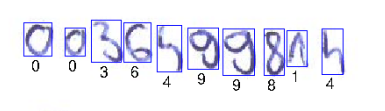
\includegraphics[scale=1.0]{uvod.png}
			\caption{Pregled problema}
		\end{figure}
		%\item Glavni problemi:
		%\begin{itemize}
		%		\item svaka osoba ima specifičan rukopis
		%		\item slabo otisnute konture nakon skeniranja (obična olovka, kemijska olovka, tehnička olovka)
		%		\item distorzije na skeniranom papiru $\rightarrow$ šum se lokalizira kao znamenka
		%		\item konture znamenaka mogu se međusobno preklapati $\rightarrow$ pogrešno označavanje dvije ili više znamenaka unutar jednog okvira 
		%\end{itemize}
	\end{itemize}
\end{frame}

%------------------------------------------------
\section{Pristup problemu}
%------------------------------------------------

\begin{frame}
	\frametitle{Pristup problemu}
	\begin{figure}[h]
		\centering
		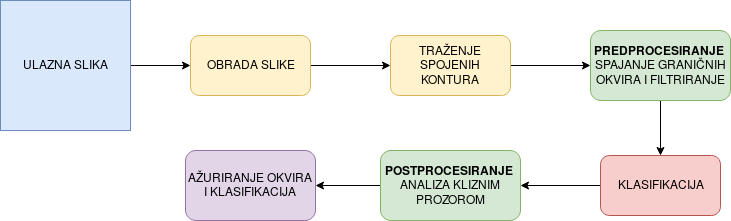
\includegraphics[scale=0.45]{system_arhitecture.png}
		\caption{Tok obrade ulazne slike kroz izgrađeni sustav}
	\end{figure}
\end{frame}

\subsection{Obrada slike}
\begin{frame}
	\frametitle{Obrada slike}
	
		\begin{itemize}
			\item Pretpostavka: ulazna slika sastoji se od dvije klase slikovnih elemenata \\
			\item Koraci:
			\begin{itemize}
				\item \textbf{pretvorba slike u sive nijanse} temeljeno na ljudskoj percepciji boja
				\item \textbf{binarizacija} $\rightarrow$ Otsuova metoda 
				\item \textbf{dilatacija} odnosno operacija podebljavanja kontura
				\item \textbf{interpolacija} $\rightarrow$  metoda najbližeg susjeda 
				\item \textbf{translacija} $\rightarrow$  metoda centra mase
			\end{itemize}
		\end{itemize}
\end{frame}


\subsection{Pronalazak spojenih kontura}
\begin{frame}
	\frametitle{Pronalazak spojenih kontura}
		\begin{itemize}
			\item Lokalizacije pojedine znamenke vrši se pronalaskom spojenih kontura $\rightarrow$ \textit{Connected Component Labeling}
			\item Problem preklapajućih i spojenih kontura znamenaka (\textbf{analiza kliznim prozorom}) i problem podjele konture na više dijelova (\textbf{dilatacija})
		\end{itemize}

\begin{figure}
	\begin{subfigure}[t]{.4\textwidth}
		\centering
		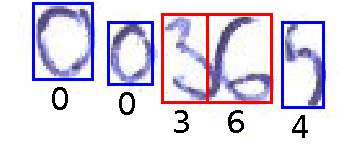
\includegraphics[width=\linewidth]{spojene_konture.png}
		\caption{Primjer spojenih kontura}
	\end{subfigure}
	\hfill
	\begin{subfigure}[t]{.4\textwidth}
		\centering
		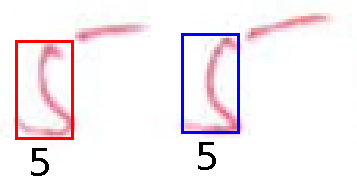
\includegraphics[width=\linewidth]{error_3.png}
		\caption{Primjer pogrešne lokalizacije}
	\end{subfigure}
\end{figure}
\end{frame}

\section{Predprocesiranje}
\begin{frame}
	\frametitle{Predprocesiranje}
	Cilj
	\begin{itemize}
		\item \textbf{eliminiranje šumova}
		\item \textbf{spajanje okvira} koji vjerojatno čine jednu znamenku
	\end{itemize}
	Opis
	\begin{itemize}
			\item u potpunosti temeljen na \textit{a priori} znanju o tome kako čovjek piše identifikatore 
			\item na temelju \textbf{udaljenosti između okvira}, \textbf{omjeru širina i visina} te na temelju odnosa \textbf{visine i širine potencijalno spojenog okvira} i \textbf{prosječne visine i širine svih okvira} vrši spajanja
			\item eliminira šumove na temelju \textbf{prosječne visine svih okvira}
	\end{itemize}

\end{frame}

%------------------------------------------------

\section{Klasifikacija}
\subsection{Arhitektura neuronske mreže}
\begin{frame}
	\frametitle{Duboki model}
	\begin{itemize}
		\item implementiran koristeći radni okvir za duboko učenje \textit{DeepLearning4j}
		\item  baza rukom pisanih identifikatora je izgrađena iz uzoraka od desetak različitih autora
		\item skup za učenje se sastojao od 2371 slike, a skup za ispitivanje od 402 slike
		\item učenje je provedeno kroz 30 epoha, u mini-grupama po 54 uzorka
		\item težine su inicijalizirane koristeći \textbf{Xavierovu} inicijalizaciju:  \begin{equation}
		W_{i, j} \sim \mathcal{N}(0, \frac{2}{n_{in} + n_{out}})
		\end{equation} 
		\item učenje stohastičkim gradijentnim spustom (SGD) s Nesterovim momentom
		\item L2 regularizacija
	\end{itemize}
\end{frame}

\begin{frame}
	\frametitle{Arhitektura dubokog konvolucijskog modela}
	\begin{itemize}
		\item Ukupno 6 slojeva i $1\,385\,130$ parametara 
	\end{itemize}

	\begin{figure}[h]
		\centering
		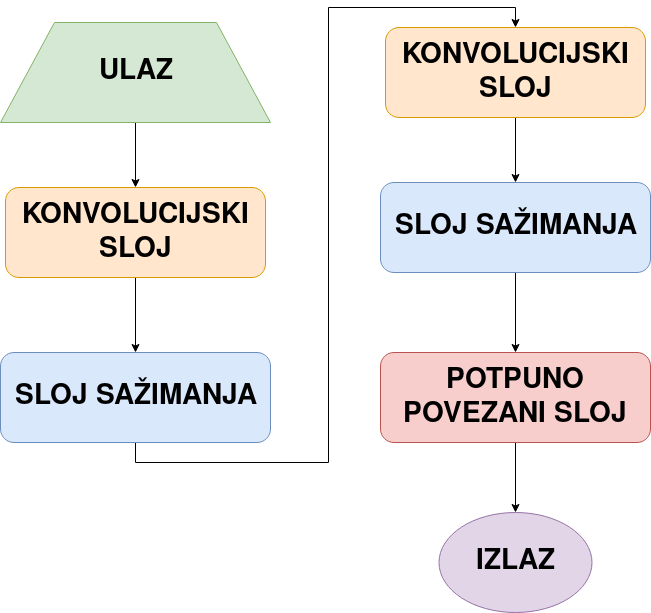
\includegraphics[scale=0.24]{arhitektura_neuronske.png}
		\caption{Arhitektura izgrađenog konvolucijskog modela}
	\end{figure}
\end{frame}
\subsection{Rezultati}

\begin{frame}
\frametitle{Matrica zabune i evaluacije (makro uprosječena)}

\begin{table}[h]
	\centering
	\begin{tabular}{lllllllllll}
		& \cellcolor[HTML]{FFFFFF}{\color[HTML]{333333} 0} & 1 & 2 & 3 & 4 & 5 & 6 & 7 & 8 & 9 \\ \cline{2-11}
		\multicolumn{1}{l|}{0=0} & \multicolumn{1}{l|}{\cellcolor[HTML]{FFCB2F}39} & \multicolumn{1}{l|}{0} & \multicolumn{1}{l|}{0} & \multicolumn{1}{l|}{0} & \multicolumn{1}{l|}{0} & \multicolumn{1}{l|}{0} & \multicolumn{1}{l|}{0} & \multicolumn{1}{l|}{0} & \multicolumn{1}{l|}{1} & \multicolumn{1}{l|}{0} \\ \cline{2-11}
		\multicolumn{1}{l|}{1=1} & \multicolumn{1}{l|}{0} & \multicolumn{1}{l|}{\cellcolor[HTML]{FFCB2F}41} & \multicolumn{1}{l|}{0} & \multicolumn{1}{l|}{0} & \multicolumn{1}{l|}{0} & \multicolumn{1}{l|}{0} & \multicolumn{1}{l|}{0} & \multicolumn{1}{l|}{0} & \multicolumn{1}{l|}{0} & \multicolumn{1}{l|}{0} \\ \cline{2-11}
		\multicolumn{1}{l|}{2=2} & \multicolumn{1}{l|}{0} & \multicolumn{1}{l|}{0} & \multicolumn{1}{l|}{\cellcolor[HTML]{FFCB2F}40} & \multicolumn{1}{l|}{0} & \multicolumn{1}{l|}{0} & \multicolumn{1}{l|}{0} & \multicolumn{1}{l|}{0} & \multicolumn{1}{l|}{0} & \multicolumn{1}{l|}{0} & \multicolumn{1}{l|}{0} \\ \cline{2-11}
		\multicolumn{1}{l|}{3=3} & \multicolumn{1}{l|}{0} & \multicolumn{1}{l|}{0} & \multicolumn{1}{l|}{0} & \multicolumn{1}{l|}{\cellcolor[HTML]{FFCB2F}37} & \multicolumn{1}{l|}{0} & \multicolumn{1}{l|}{0} & \multicolumn{1}{l|}{0} & \multicolumn{1}{l|}{0} & \multicolumn{1}{l|}{0} & \multicolumn{1}{l|}{3} \\ \cline{2-11}
		\multicolumn{1}{l|}{4=4} & \multicolumn{1}{l|}{0} & \multicolumn{1}{l|}{0} & \multicolumn{1}{l|}{0} & \multicolumn{1}{l|}{0} & \multicolumn{1}{l|}{\cellcolor[HTML]{FFCB2F}40} & \multicolumn{1}{l|}{0} & \multicolumn{1}{l|}{0} & \multicolumn{1}{l|}{0} & \multicolumn{1}{l|}{0} & \multicolumn{1}{l|}{0} \\ \cline{2-11}
		\multicolumn{1}{l|}{5=5} & \multicolumn{1}{l|}{0} & \multicolumn{1}{l|}{0} & \multicolumn{1}{l|}{0} & \multicolumn{1}{l|}{0} & \multicolumn{1}{l|}{0} & \multicolumn{1}{l|}{\cellcolor[HTML]{FFCB2F}36} & \multicolumn{1}{l|}{4} & \multicolumn{1}{l|}{0} & \multicolumn{1}{l|}{0} & \multicolumn{1}{l|}{0} \\ \cline{2-11}
		\multicolumn{1}{l|}{6=6} & \multicolumn{1}{l|}{0} & \multicolumn{1}{l|}{0} & \multicolumn{1}{l|}{0} & \multicolumn{1}{l|}{0} & \multicolumn{1}{l|}{2} & \multicolumn{1}{l|}{0} & \multicolumn{1}{l|}{\cellcolor[HTML]{FFCB2F}38} & \multicolumn{1}{l|}{0} & \multicolumn{1}{l|}{0} & \multicolumn{1}{l|}{0} \\ \cline{2-11}
		\multicolumn{1}{l|}{7=7} & \multicolumn{1}{l|}{0} & \multicolumn{1}{l|}{0} & \multicolumn{1}{l|}{0} & \multicolumn{1}{l|}{0} & \multicolumn{1}{l|}{0} & \multicolumn{1}{l|}{0} & \multicolumn{1}{l|}{0} & \multicolumn{1}{l|}{\cellcolor[HTML]{FFCB2F}41} & \multicolumn{1}{l|}{0} & \multicolumn{1}{l|}{0} \\ \cline{2-11}
		\multicolumn{1}{l|}{8=8} & \multicolumn{1}{l|}{0} & \multicolumn{1}{l|}{0} & \multicolumn{1}{l|}{0} & \multicolumn{1}{l|}{0} & \multicolumn{1}{l|}{0} & \multicolumn{1}{l|}{0} & \multicolumn{1}{l|}{0} & \multicolumn{1}{l|}{0} & \multicolumn{1}{l|}{\cellcolor[HTML]{FFCB2F}40} & \multicolumn{1}{l|}{0} \\ \cline{2-11}
		\multicolumn{1}{l|}{9=9} & \multicolumn{1}{l|}{0} & \multicolumn{1}{l|}{0} & \multicolumn{1}{l|}{0} & \multicolumn{1}{l|}{0} & \multicolumn{1}{l|}{3} & \multicolumn{1}{l|}{0} & \multicolumn{1}{l|}{0} & \multicolumn{1}{l|}{0} & \multicolumn{1}{l|}{0} & \multicolumn{1}{l|}{\cellcolor[HTML]{FFCB2F}37} \\ \cline{2-11}
	\end{tabular}
\end{table}

\begin{table}[h]
	\centering
	\begin{tabular}{|c|
			>{\columncolor[HTML]{FFCB2F}}c |}
		\hline
		Točnost & {\color[HTML]{333333} 0.9677} \\ \hline
		Preciznost & 0.9694 \\ \hline
		Odziv & 0.9675 \\ \hline
		F1 & 0.9676 \\ \hline
	\end{tabular}
\end{table}
\end{frame}

%------------------------------------------------
\section{Postprocesiranje}
\begin{frame}
\frametitle{Postprocesiranje}
Cilj
\begin{itemize}
	\item predviđanje i razrješavanje pogrešno lokaliziranih/klasificiranih znamenaka
\end{itemize}
Uvjeti da bi se okvir razmatrao kao pogrešno lokaliziran/klasificiran:
\begin{itemize}
	\item širina okvira mora biti barem 1.5 puta veća od prosječne širine svih okvira
	\item sigurnost (engl. \textit{confidence}) klasifikatora u odluku mora biti manja od 50\% i zbunjenost (engl. \textit{perplexity}) mora biti veća od eksperimentalno dobivene vrijednosti
\end{itemize}
\begin{block}{Zbunjenost modela}
Zbunjenost diskretne vjerojatnosne distribucije $p$ definiramo preko mjere nesigurnosti ili neodređenosti modela, odnosno preko entropije kao 
\begin{equation}
2^{H(p)} = 2 ^ {- \sum_{x}^{}p(x)\log_{2}p(x)}.
\end{equation}
\end{block}
\end{frame}

\begin{frame}
	\frametitle{Postprocesiranje}
	Opis algoritma razrješavanja pogrešno lokaliziranih/klasificiranih okvira
	\begin{itemize}
		\item \textbf{metodom kliznog prozora} vrši se analiza okvira
		\item veličine kliznog prozora su \textbf{dinamičke}
		\item različitim veličinama kliznog prozora pokušava se podijeliti okvir kako bi postigli minimalnu zbunjenost modela
	\end{itemize}
\begin{block}{Izraz za traženje podjele okvira s najmanjom zbunjenosti}
	\begin{equation}
		Utjecaj = \sum_{i = 0}^{broj\ okvira\ -\ 1} zbunjenost_{i}^2 \cdot  {\rm e}^{-i}.
	\end{equation}	
\end{block}
\end{frame}

%------------------------------------------------

\section{Izgrađeni sustav}

\begin{frame}
	\frametitle{Izgrađeni sustav}
	\begin{figure}[h]
		\centering
		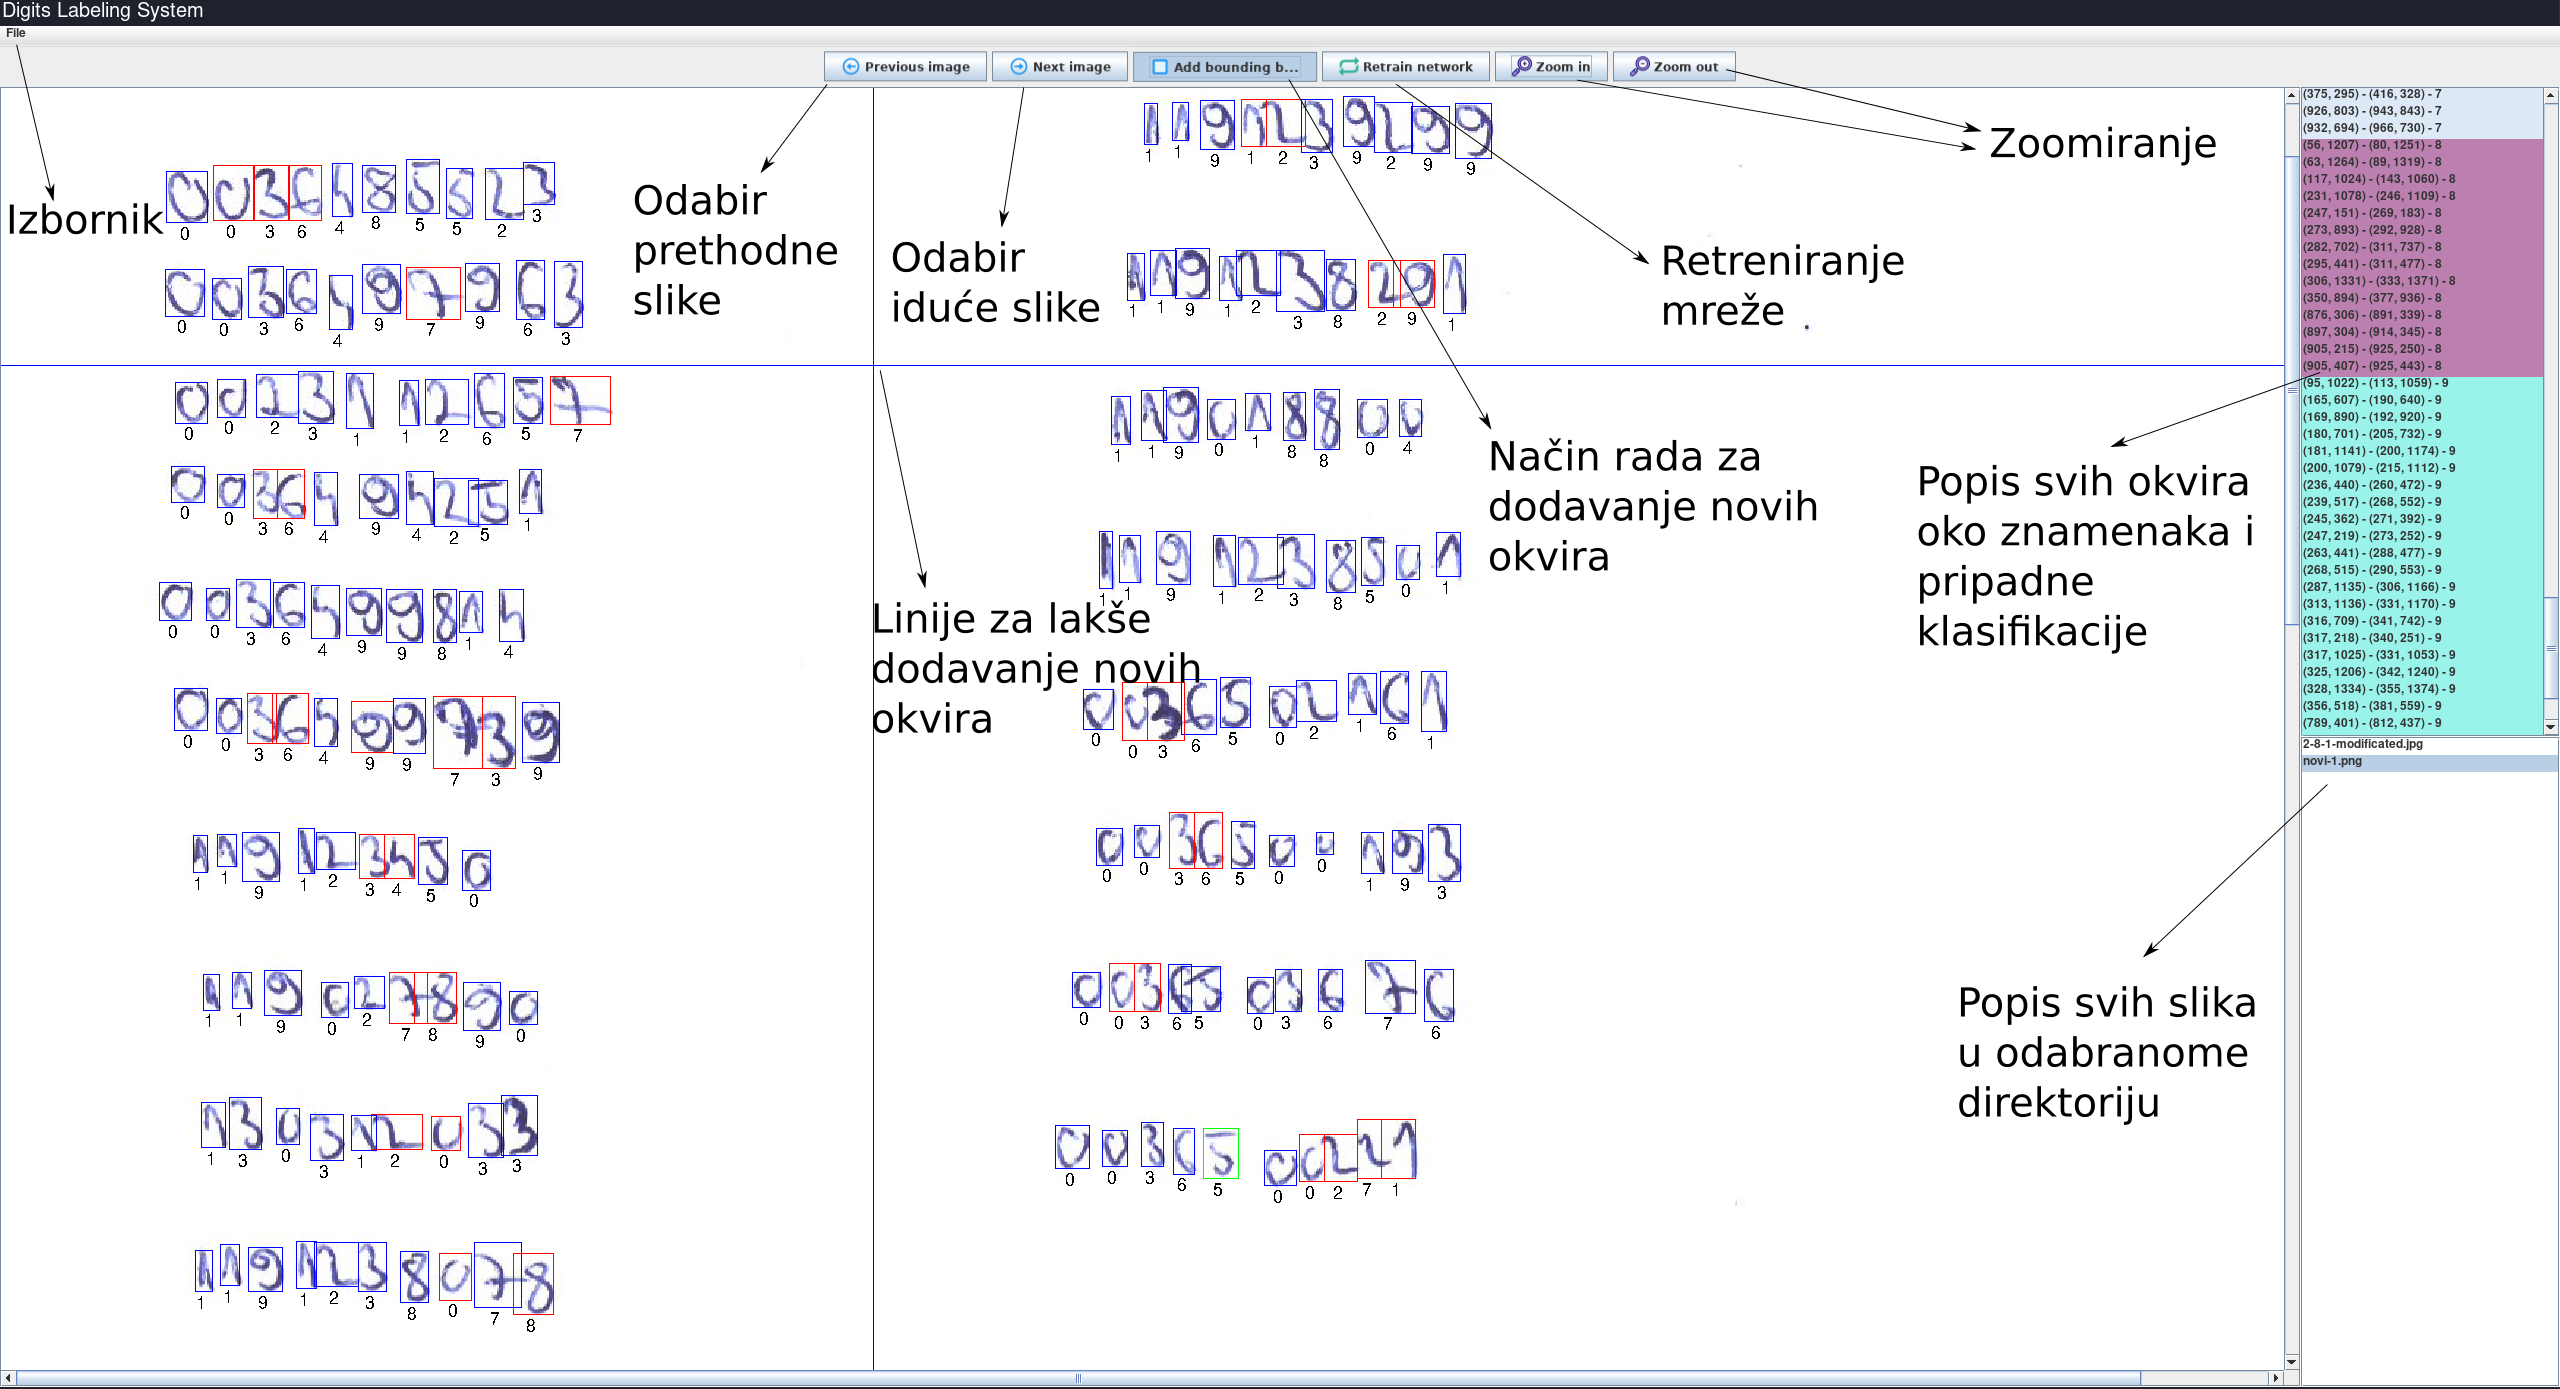
\includegraphics[scale=0.18]{master_detail.png}
		\caption{Prikaz glavnog ekrana aplikacije}
	\end{figure}
\end{frame}

\section{Rezultati}
\begin{frame}
	\frametitle{Rezultati}
	\begin{itemize}
		\item Na ulaznim uzorcima gdje su znamenke razmaknute sustav s visokim postotkom uspješnosti vrši lokalizaciju i klasifikaciju
		\item Izradom postprocesora pokazuje se značajan napredak na ulaznim slikama s gusto napisanim brojevima
		\item Na uzorku od 230 znamenaka (23 studentska identifikatora) 8 znamenaka je sustav krivo segmentirao (3.48\%), dok je 6 znamenaka djelomično krivo segmentirao (2.61\%), no dovoljno dobro za uspješnu klasifikaciju
	\end{itemize}
\end{frame}

\begin{frame}
	\frametitle{Primjer pogrešaka prilikom segmentacije i klasifikacije}
	\begin{figure}
		\begin{subfigure}[t]{.4\textwidth}
			\centering
			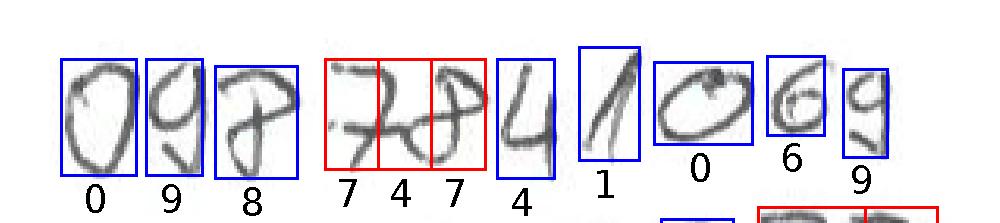
\includegraphics[width=\linewidth]{error_2.png}
			\caption{Primjer pogrešne separacije okvira na više manjih}
			\label{error1}
		\end{subfigure}
		\hfill
		\begin{subfigure}[t]{.4\textwidth}
			\centering
			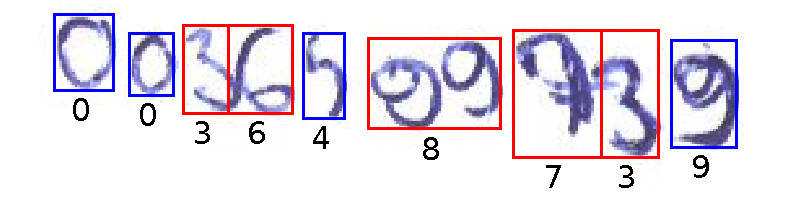
\includegraphics[width=\linewidth]{postprocesor.png}
			\caption{Primjer okvira koji sadrži dvije znamenke}
			\label{error2}
		\end{subfigure}
		
		\medskip
		
		\begin{subfigure}[t]{.4\textwidth}
			\centering
			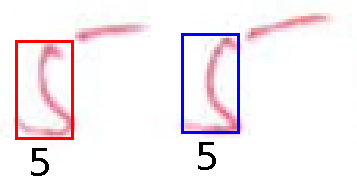
\includegraphics[width=\linewidth]{error_3.png}
			\caption{Primjer pogrešne segmentacije zbog načina pisanja}
			\label{error3}
		\end{subfigure}
		\hfill
		\begin{subfigure}[t]{.4\textwidth}
			\centering
			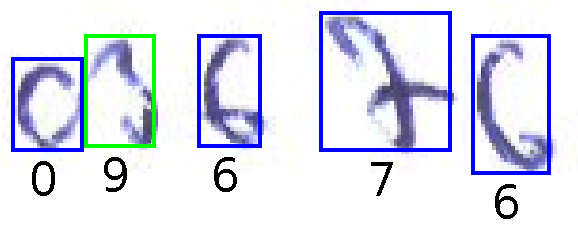
\includegraphics[width=\linewidth]{error_4.png}
			\caption{Primjer pogrešne klasifikacije}
			\label{error4}
		\end{subfigure}
		\caption{Primjer pogrešaka prilikom segmentacije i klasifikacije}
	\end{figure}
\end{frame}

\section{Zaključak}
\begin{frame}
	\frametitle{Zaključak}
	\begin{itemize}
		\item Mješavinom zaključaka stečenim \textbf{učenjem klasifikatora} i \textbf{matematičkim pretpostavkama o problemu} sustav se vrlo dobro nosio s problemima lokalizacije i klasifikacije
		\item Daljnja unapređenja treba usmjeriti ka sustavu za \textbf{postprocesiranje} (\textbf{metoda kliznog prozora})
		\item Povećanjem skupa uzoraka za učenje klasifikator postaje još robusniji i kvalitetnije se nosi s problemima
		\item Eksperimentiranjem nad matematički modeliranim znanjem možemo fino ugađati sustav i dodavanjem novog znanja poboljšati rad sustava
		\end{itemize}
	\end{frame}

%------------------------------------------------
%------------------------------------------------

\begin{frame} 
\Huge{\centerline{Hvala na pažnji!}}
\end{frame}

\begin{frame}[noframenumbering]
	\frametitle{Konvolucija}
	\begin{figure}[h]
		\centering
		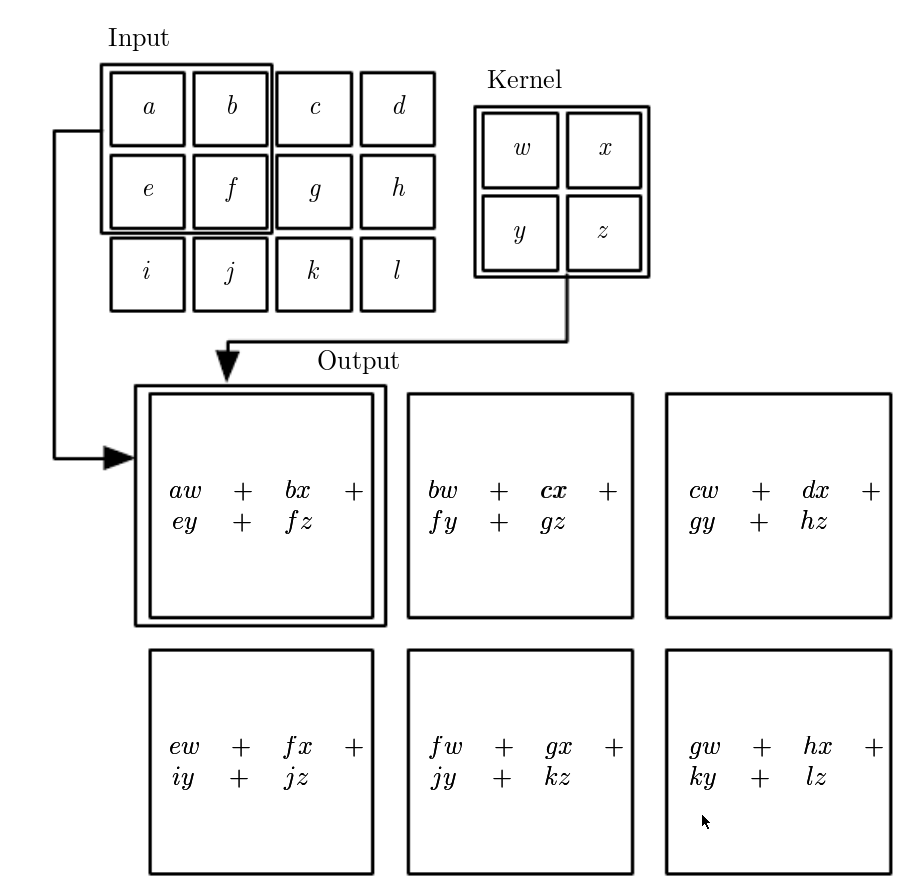
\includegraphics[scale=0.3]{convolution.png}
		\caption{Konvolucija 2D ulaza i jezgre}
	\end{figure}
\end{frame}

\begin{frame}[noframenumbering]
	\frametitle{Specifičnosti dubokih modela}
	\begin{itemize}
		\item Koristeći \textbf{lokalnu interakciju} potrebno je naučiti manje parametara s istom količinom označenih podataka
		\item \textbf{Dijeljenje parametara} omogućuje da svi izlazi dijele jedan te isti skup parametara $\rightarrow$ manji model koji je teže prenaučiti
		\item \textbf{Sažimanjem} dobivamo reprezentaciju koja je približno invarijantna na male translacije u ulazu (fokusiramo se na postojanje objekta, a ne na točnu lokaciju)
	\end{itemize}
\end{frame}

\begin{frame}[noframenumbering]
	\frametitle{Vrednovanje klasifikatora}
	\begin{itemize}
		\item \textbf{Točnost} definiramo kao omjer ispravno klasificiranih primjera i ukupnog broja primjera:
		$A_{cc} = \frac{TP + TN}{N} = \frac{TP + TN}{TP + TN + FP + FN}$
		\item \textbf{Preciznost} je definirana izrazom: $P = \frac{TP}{TP + FP}$
		\item \textbf{Odziv} je definiran omjerom broja primjera koje je klasifikator označio kao pozitivne i ukupnog broja pozitivnih primjera:
		$R = \frac{TP}{TP + FN}$
		\item \textbf{F1} mjeru definiramo kao harmonijsku sredinu između preciznosti i odziva:
		$F1 = \frac{2}{\frac{1}{P} + \frac{1}{R}} = \frac{2PR}{P + R}$
	\end{itemize}
\end{frame}

\begin{frame}[noframenumbering]
	\frametitle{Makro i mikro mjera}
	\begin{figure}[h]
		\centering
		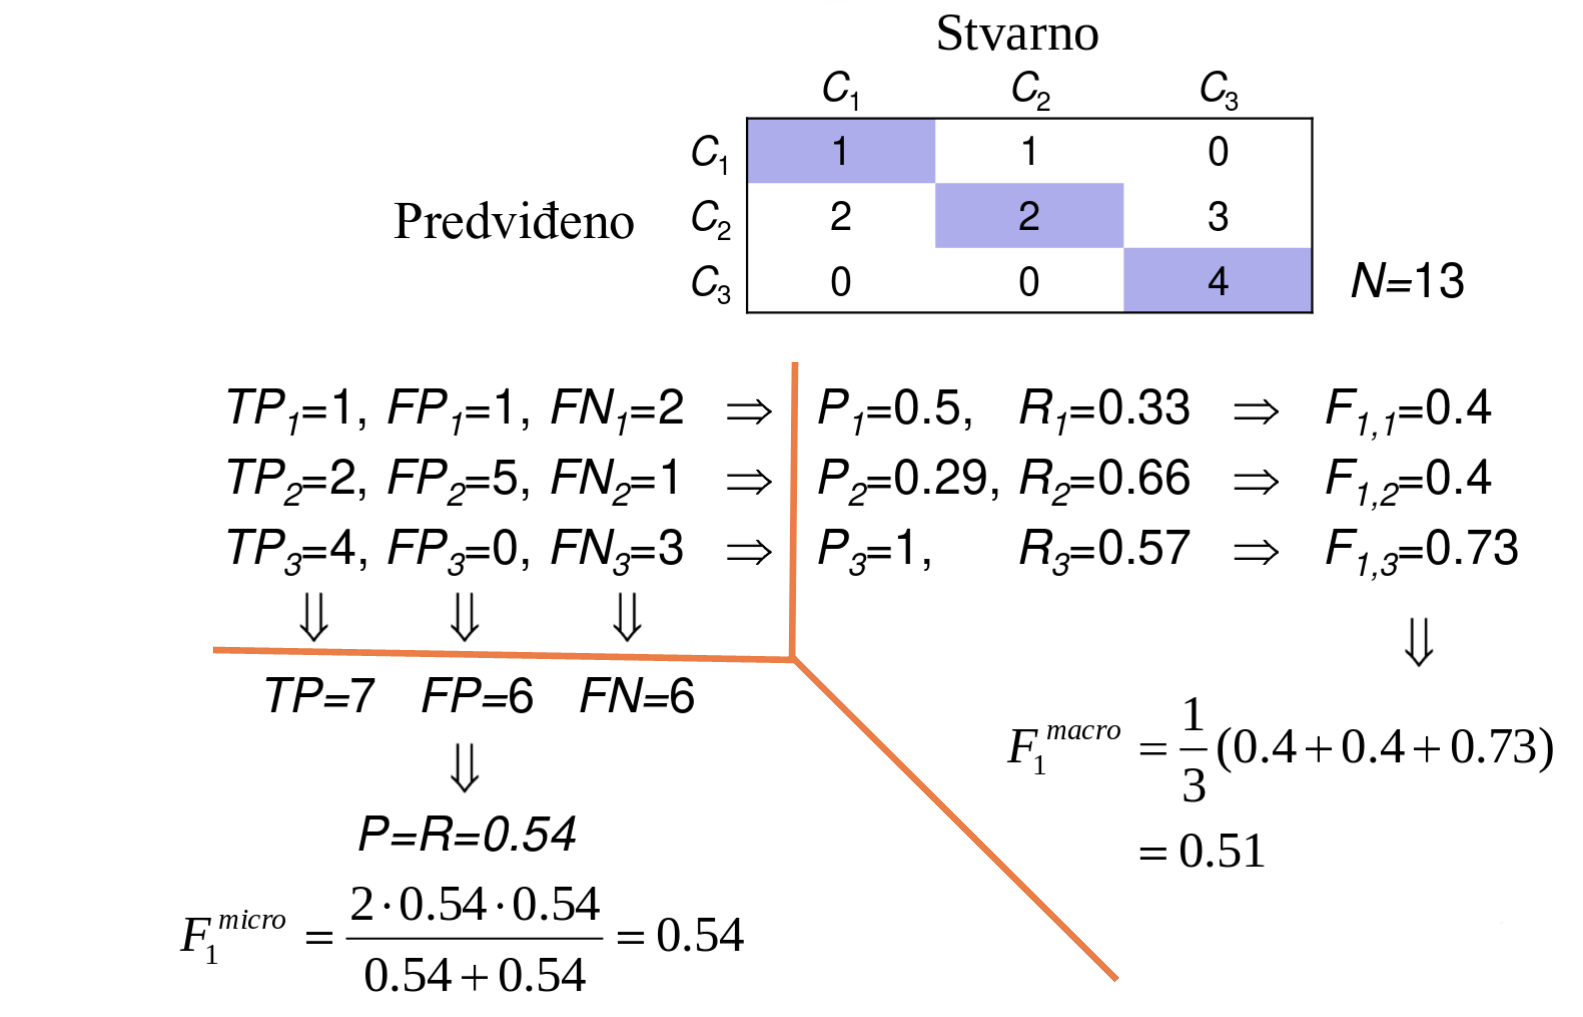
\includegraphics[scale=0.2]{makro_mikro.png}
	\end{figure}
\end{frame}

\begin{frame}[noframenumbering]
	\frametitle{Makro vs. mikro mjera}
	\begin{itemize}
		\item Makro-$F_1$ sve klase tretira jednako
		\begin{itemize}
			\item zbog toga primjeri iz malih klasa imaju veći utjecaj na mjeru nego što bi imali kod mjere mikro-$F_1$
			\item razlika je vidljiva kod neuravnoteženih skupova
			\item 	\begin{figure}[h]
				\centering
				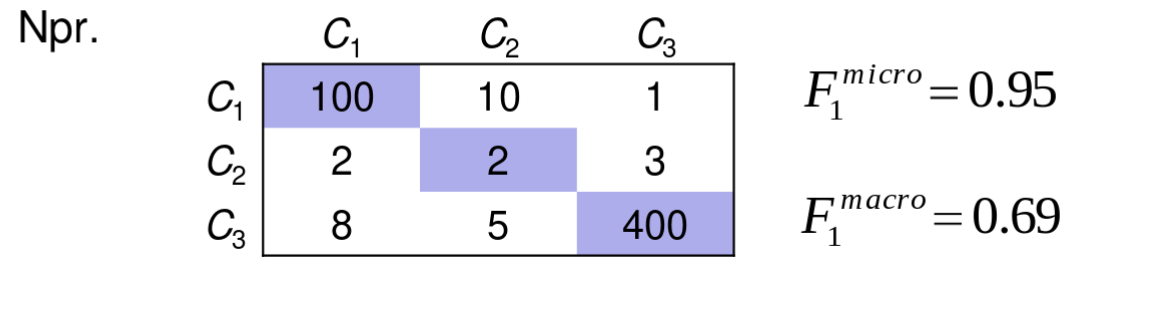
\includegraphics[scale=0.3]{makro_mikro_primjer.png}
			\end{figure}
		\end{itemize} 
		\item makro-$F_1$ je tipično manji od mikro-$F_1$
		\begin{itemize}
			\item zato jer je na slabo zastupljenim klasama klasifikacija tipično lošija
		\end{itemize}
	\end{itemize}
\end{frame}

\begin{frame}[noframenumbering]
	\frametitle{Pronalazak spojenih kontura}
	\begin{figure}[H]
		\begin{center}
			
\begin{tikzpicture}
			[%%%%%%%%%%%%%%%%%%%%%%%%%%%%%%
			box/.style={rectangle,draw=black,thick, minimum size=1cm},
			]%%%%%%%%%%%%%%%%%%%%%%%%%%%%%%
			
			\foreach \x in {0,1,...,7}{
				\foreach \y in {0,1,...,7}
				\node[box] at (\x,\y){};
			}
			\node[box,fill=black] at (0,2){};
			\node[box,fill=black ] at (0,4){};
			\node[box,fill=black] at (1,2){};
			\node[box,fill=black ] at (1,4){};
			\node[box,fill=black] at (2,2){};
			\node[box,fill=black ] at (2,4){};
			\node[box,fill=black] at (2,6){};
			\node[box,fill=black ] at (2,7){};
			\node[box,fill=black] at (3,4){};
			\node[box,fill=black ] at (4,0){};
			\node[box,fill=black ] at (4,1){};
			\node[box,fill=black ] at (4,2){};
			\node[box,fill=black ] at (4,3){};
			\node[box,fill=black ] at (4,4){};
			\node[box,fill=black ] at (4,5){};
			\node[box,fill=black ] at (4,6){};
			\node[box,fill=black ] at (5,1){};
			\node[box,fill=black ] at (5,4){};
			\node[box,fill=black ] at (5,5){};
			\node[box,fill=black ] at (6,1){};
			\node[box,fill=black ] at (6,2){};
			\node[box,fill=black ] at (6,3){};
			\node[box,fill=black ] at (6,4){};
			\node[box,fill=black ] at (6,5){};
			\node[box,fill=black ] at (6,6){};
			\node[box,fill=black ] at (6,7){};
			\end{tikzpicture}
		\end{center}
	\end{figure}
\end{frame}

\begin{frame}[noframenumbering]
	\frametitle{Pronalazak spojenih kontura}
	\begin{figure}[H]
		\begin{center}
			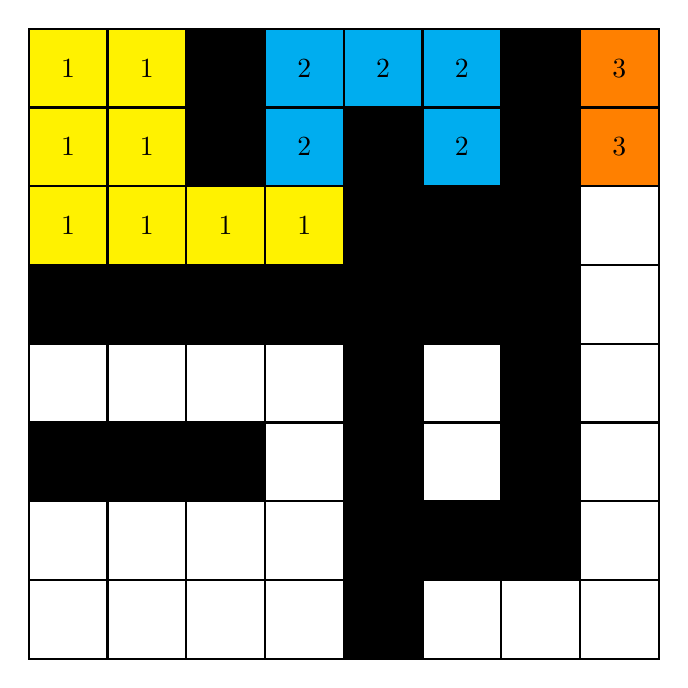
\begin{tikzpicture}
			[%%%%%%%%%%%%%%%%%%%%%%%%%%%%%%
			box/.style={rectangle,draw=black,thick, minimum size=1cm},
			]%%%%%%%%%%%%%%%%%%%%%%%%%%%%%%
			
			\foreach \x in {0,1,...,7}{
				\foreach \y in {0,1,...,7}
				\node[box] at (\x,\y){};
			}
			\node[box,fill=yellow] at (0,7){1};
			\node[box,fill=yellow] at (0,6){1};
			\node[box,fill=yellow] at (0,5){1};
			\node[box,fill=yellow ] at (1,7){1};
			\node[box,fill=yellow] at (1,6){1};
			\node[box,fill=yellow ] at (1,5){1};
			\node[box,fill=yellow] at (2,5){1};
			\node[box,fill=yellow ] at (3,5){1};
			
			\node[box,fill=cyan] at (3,7){2};
			\node[box,fill=cyan ] at (3,6){2};
			\node[box,fill=cyan] at (4,7){2};
			\node[box,fill=cyan ] at (5,7){2};
			\node[box,fill=cyan] at (5,6){2};
			
			
			\node[box,fill=orange] at (7,7){3};
			\node[box,fill=orange ] at (7,6){3};
			
			\node[box,fill=black] at (0,2){};
			\node[box,fill=black ] at (0,4){};
			\node[box,fill=black] at (1,2){};
			\node[box,fill=black ] at (1,4){};
			\node[box,fill=black] at (2,2){};
			\node[box,fill=black ] at (2,4){};
			\node[box,fill=black] at (2,6){};
			\node[box,fill=black ] at (2,7){};
			\node[box,fill=black] at (3,4){};
			\node[box,fill=black ] at (4,0){};
			\node[box,fill=black ] at (4,1){};
			\node[box,fill=black ] at (4,2){};
			\node[box,fill=black ] at (4,3){};
			\node[box,fill=black ] at (4,4){};
			\node[box,fill=black ] at (4,5){};
			\node[box,fill=black ] at (4,6){};
			\node[box,fill=black ] at (5,1){};
			\node[box,fill=black ] at (5,4){};
			\node[box,fill=black ] at (5,5){};
			\node[box,fill=black ] at (6,1){};
			\node[box,fill=black ] at (6,2){};
			\node[box,fill=black ] at (6,3){};
			\node[box,fill=black ] at (6,4){};
			\node[box,fill=black ] at (6,5){};
			\node[box,fill=black ] at (6,6){};
			\node[box,fill=black ] at (6,7){};
			\end{tikzpicture}
		\end{center}
	\end{figure}
\end{frame}

\begin{frame}[noframenumbering]
	\frametitle{Pronalazak spojenih kontura}
	\begin{figure}[H]
		\begin{center}
			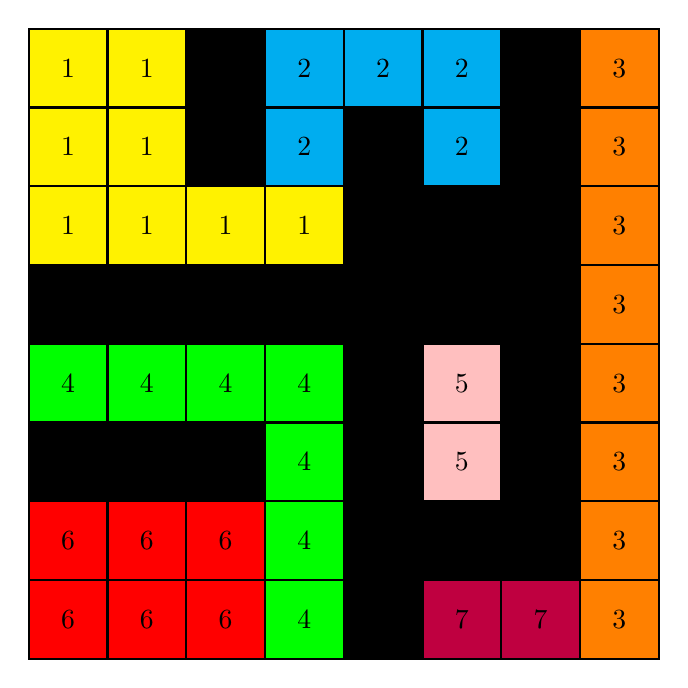
\begin{tikzpicture}
			[%%%%%%%%%%%%%%%%%%%%%%%%%%%%%%
			box/.style={rectangle,draw=black,thick, minimum size=1cm},
			]%%%%%%%%%%%%%%%%%%%%%%%%%%%%%%
			
			\foreach \x in {0,1,...,7}{
				\foreach \y in {0,1,...,7}
				\node[box] at (\x,\y){};
			}
			\node[box,fill=yellow] at (0,7){1};
			\node[box,fill=yellow] at (0,6){1};
			\node[box,fill=yellow] at (0,5){1};
			\node[box,fill=yellow ] at (1,7){1};
			\node[box,fill=yellow] at (1,6){1};
			\node[box,fill=yellow ] at (1,5){1};
			\node[box,fill=yellow] at (2,5){1};
			\node[box,fill=yellow ] at (3,5){1};
			
			\node[box,fill=cyan] at (3,7){2};
			\node[box,fill=cyan ] at (3,6){2};
			\node[box,fill=cyan] at (4,7){2};
			\node[box,fill=cyan ] at (5,7){2};
			\node[box,fill=cyan] at (5,6){2};
			
			
			\node[box,fill=orange] at (7,7){3};
			\node[box,fill=orange ] at (7,6){3};
			\node[box,fill=orange] at (7,5){3};
			\node[box,fill=orange ] at (7,4){3};
			\node[box,fill=orange] at (7,3){3};
			\node[box,fill=orange] at (7,2){3};
			\node[box,fill=orange] at (7,1){3};
			\node[box,fill=orange] at (7,0){3};
			
			\node[box,fill=purple] at (5,0){7};
			\node[box,fill=purple] at (6,0){7};
			
			\node[box,fill=red] at (0,0){6};
			\node[box,fill=red] at (0,1){6};
			\node[box,fill=red] at (1,0){6};
			\node[box,fill=red] at (1,1){6};
			\node[box,fill=red] at (2,0){6};
			\node[box,fill=red] at (2,1){6};
			
			\node[box,fill=green] at (0,3){4};
			\node[box,fill=green] at (1,3){4};
			\node[box,fill=green] at (2,3){4};
			\node[box,fill=green] at (3,3){4};
			\node[box,fill=green] at (3,2){4};
			\node[box,fill=green] at (3,1){4};
			\node[box,fill=green] at (3,0){4};
			
			\node[box,fill=pink] at (5,3){5};
			\node[box,fill=pink] at (5,2){5};
			
			\node[box,fill=black] at (0,2){};
			\node[box,fill=black ] at (0,4){};
			\node[box,fill=black] at (1,2){};
			\node[box,fill=black ] at (1,4){};
			\node[box,fill=black] at (2,2){};
			\node[box,fill=black ] at (2,4){};
			\node[box,fill=black] at (2,6){};
			\node[box,fill=black ] at (2,7){};
			\node[box,fill=black] at (3,4){};
			\node[box,fill=black ] at (4,0){};
			\node[box,fill=black ] at (4,1){};
			\node[box,fill=black ] at (4,2){};
			\node[box,fill=black ] at (4,3){};
			\node[box,fill=black ] at (4,4){};
			\node[box,fill=black ] at (4,5){};
			\node[box,fill=black ] at (4,6){};
			\node[box,fill=black ] at (5,1){};
			\node[box,fill=black ] at (5,4){};
			\node[box,fill=black ] at (5,5){};
			\node[box,fill=black ] at (6,1){};
			\node[box,fill=black ] at (6,2){};
			\node[box,fill=black ] at (6,3){};
			\node[box,fill=black ] at (6,4){};
			\node[box,fill=black ] at (6,5){};
			\node[box,fill=black ] at (6,6){};
			\node[box,fill=black ] at (6,7){};
			\end{tikzpicture}
		\end{center}
	\end{figure}
\end{frame}

\begin{frame}[noframenumbering]
	\frametitle{Pronalazak spojenih kontura}
\begin{figure}[H]
	\begin{center}
		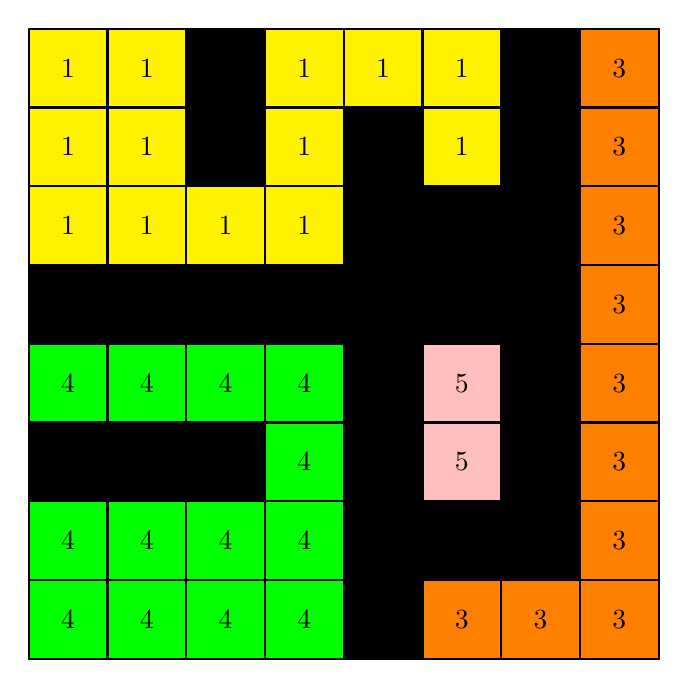
\begin{tikzpicture}
		[%%%%%%%%%%%%%%%%%%%%%%%%%%%%%%
		box/.style={rectangle,draw=black,thick, minimum size=1cm},
		]%%%%%%%%%%%%%%%%%%%%%%%%%%%%%%
		
		\foreach \x in {0,1,...,7}{
			\foreach \y in {0,1,...,7}
			\node[box] at (\x,\y){};
		}
		\node[box,fill=yellow] at (0,7){1};
		\node[box,fill=yellow] at (0,6){1};
		\node[box,fill=yellow] at (0,5){1};
		\node[box,fill=yellow ] at (1,7){1};
		\node[box,fill=yellow] at (1,6){1};
		\node[box,fill=yellow ] at (1,5){1};
		\node[box,fill=yellow] at (2,5){1};
		\node[box,fill=yellow ] at (3,5){1};
		
		\node[box,fill=yellow] at (3,7){1};
		\node[box,fill=yellow ] at (3,6){1};
		\node[box,fill=yellow] at (4,7){1};
		\node[box,fill=yellow ] at (5,7){1};
		\node[box,fill=yellow] at (5,6){1};
		
		
		\node[box,fill=orange] at (7,7){3};
		\node[box,fill=orange ] at (7,6){3};
		\node[box,fill=orange] at (7,5){3};
		\node[box,fill=orange ] at (7,4){3};
		\node[box,fill=orange] at (7,3){3};
		\node[box,fill=orange] at (7,2){3};
		\node[box,fill=orange] at (7,1){3};
		\node[box,fill=orange] at (7,0){3};
		
		\node[box,fill=orange] at (5,0){3};
		\node[box,fill=orange] at (6,0){3};
		
		\node[box,fill=green] at (0,0){4};
		\node[box,fill=green] at (0,1){4};
		\node[box,fill=green] at (1,0){4};
		\node[box,fill=green] at (1,1){4};
		\node[box,fill=green] at (2,0){4};
		\node[box,fill=green] at (2,1){4};
		
		\node[box,fill=green] at (0,3){4};
		\node[box,fill=green] at (1,3){4};
		\node[box,fill=green] at (2,3){4};
		\node[box,fill=green] at (3,3){4};
		\node[box,fill=green] at (3,2){4};
		\node[box,fill=green] at (3,1){4};
		\node[box,fill=green] at (3,0){4};
		
		\node[box,fill=pink] at (5,3){5};
		\node[box,fill=pink] at (5,2){5};
		
		\node[box,fill=black] at (0,2){};
		\node[box,fill=black ] at (0,4){};
		\node[box,fill=black] at (1,2){};
		\node[box,fill=black ] at (1,4){};
		\node[box,fill=black] at (2,2){};
		\node[box,fill=black ] at (2,4){};
		\node[box,fill=black] at (2,6){};
		\node[box,fill=black ] at (2,7){};
		\node[box,fill=black] at (3,4){};
		\node[box,fill=black ] at (4,0){};
		\node[box,fill=black ] at (4,1){};
		\node[box,fill=black ] at (4,2){};
		\node[box,fill=black ] at (4,3){};
		\node[box,fill=black ] at (4,4){};
		\node[box,fill=black ] at (4,5){};
		\node[box,fill=black ] at (4,6){};
		\node[box,fill=black ] at (5,1){};
		\node[box,fill=black ] at (5,4){};
		\node[box,fill=black ] at (5,5){};
		\node[box,fill=black ] at (6,1){};
		\node[box,fill=black ] at (6,2){};
		\node[box,fill=black ] at (6,3){};
		\node[box,fill=black ] at (6,4){};
		\node[box,fill=black ] at (6,5){};
		\node[box,fill=black ] at (6,6){};
		\node[box,fill=black ] at (6,7){};
		\end{tikzpicture}
	\end{center}
\end{figure}
\end{frame}

\begin{frame}[noframenumbering]
	\frametitle{Otsuova metoda}
	\begin{figure}[h]
		\centering
		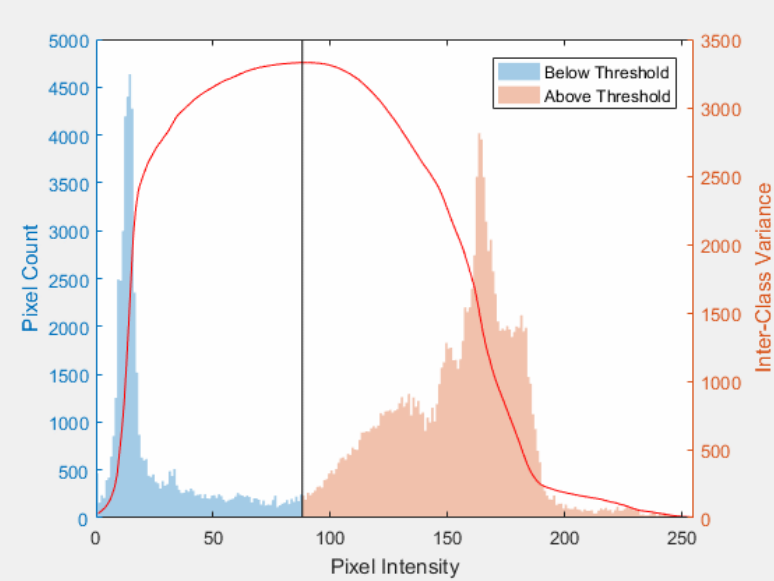
\includegraphics[scale=0.4]{otsu_method.png}
		\caption{Prikaz određivanja praga binarizacije koristeći maksimizaciju varijance između razreda }
	\end{figure}
\end{frame}

\begin{frame}[noframenumbering]
	\frametitle{Učenje s momentom}
	\begin{itemize}
		\item Ubrzavanje učenja kod šumovite procjene gradijenata i kod malih ali konzistentnih gradijenata
		\item Postupak akumulira eksponencijalno umanjujući prosjek prethodno izračunatih gradijenata i nastavlja u tome smjeru
	\end{itemize}
	\begin{equation}
		\bm{v} \leftarrow \alpha \cdot \bm{v} - \epsilon \cdot \nabla_{\bm{\theta}}(\frac{1}{m} \sum_{i=1}^{m}L(f(\bm{x}^{(i)}; \bm{\theta}), y^i )
	\end{equation}
	\begin{equation}
		\bm{\theta} \leftarrow \bm{\theta} + \bm{v}
	\end{equation}

\end{frame}

%----------------------------------------------------------------------------------------


\end{document} 